\section{Introduction}
In this chapter, we will jump into the methodology of our work. To begin, we will provide a comprehensive overview of the system. We will then proceed to explain the details in a step-by-step manner. Finally, we will showcase the implementation of our thesis.It involves several stages including data preparation, model architecture, training, and evaluation. Below is a detailed breakdown of the methodology employed in this project.
% Figure \ref{metho1} depicts the overview of our proposed Framework.

% \begin{figure}[H]
% \centering
% 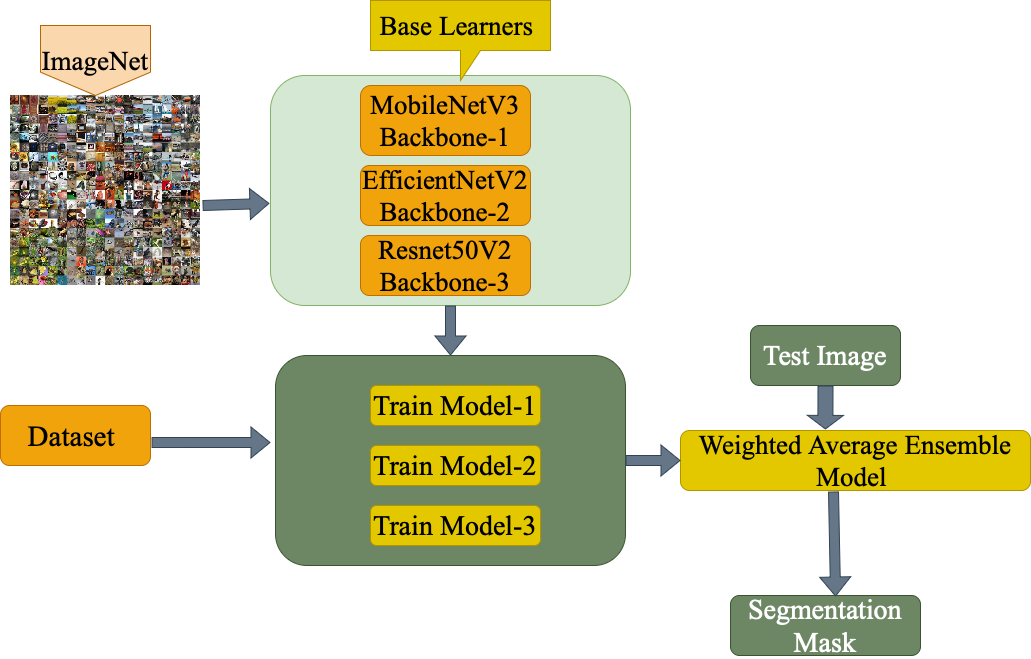
\includegraphics[width= 0.9\textwidth]{figs/first-3.png}
% \caption{Proposed Framework}
% \label{metho1}
% \end{figure}

\section{Overview of the Methodology}
The methodology for the water bodies segmentation using DeepLabV3+ with weighted avearage ensemble method is structured into several critical steps. Initially, the system setup involved installing necessary libraries and dependencies and configuring the environment for reproducibility. The dataset was then prepared by defining essential configurations such as image size, batch size, number of classes, and augmentation factors, followed by splitting it into training, validation, and test sets. Data processing involved reading and preprocessing images and masks, with functions handling resizing, normalization, and augmentations to ensure the data was in the appropriate format for model training. TensorFlow datasets were created from the images and masks, applying preprocessing functions to make the data ready for the DeepLabV3+ model. This structured approach ensures the model can be effectively trained and evaluated for the task of water segmentation. Figure \ref{metho2} depicts the overview of our proposed Methodology.



\begin{figure}[H]
\centering
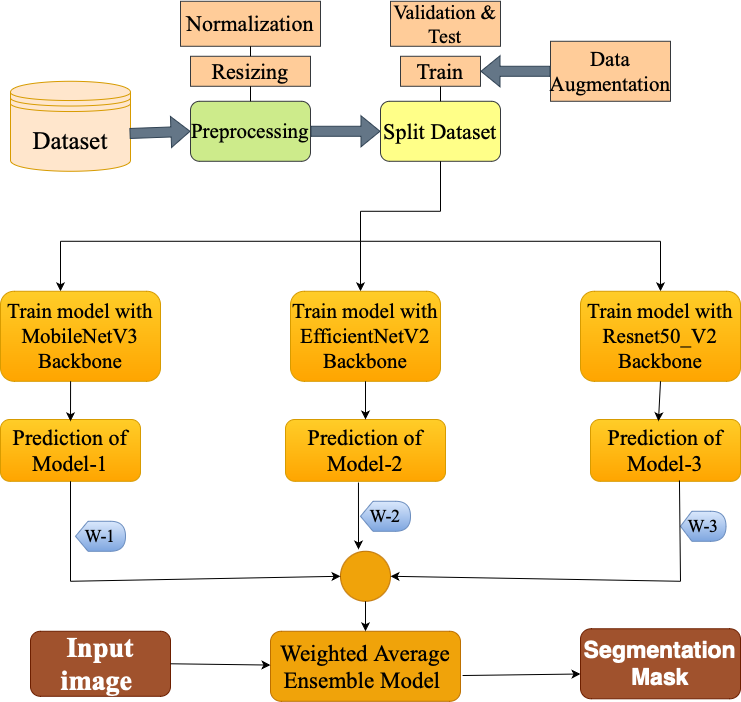
\includegraphics[width= 1\textwidth]{figs/ensemble.png}
\caption{Proposed Methodology}
\label{metho2}
\end{figure}



\subsection{Dataset Preprocessing}


\begin{enumerate}
  \item \textbf{Resizing: }In the context of preparing datasets for machine learning models, resizing is a critical preprocessing step. For this thesis, resizing involves adjusting the dimensions of the images and their corresponding segmentation masks to ensure uniformity and compatibility with the DeepLabV3+ model, which simplifies the training process. Below are the detailed steps and rationale for resizing the datasets:
  \begin{itemize}
      \item \textbf{Uniform Image Size:} Machine learning models, especially Convolutional Neural Networks (CNNs) like DeepLabV3+, require inputs of consistent size. Resizing all images and their corresponding masks to the same dimensions ensures that each input tensor has the same shape, which simplifies the training process and model architecture.
      \item \textbf{Memory and Computational Efficiency : }Resizing images to a smaller, fixed size (e.g. 256x256 pixels), which shows in \ref{res} reduces the computational load and memory usage. This makes it feasible to train the model on available hardware, especially when dealing with large datasets.
      \item \textbf{Aspect Ratio Considerations: }While resizing, it's important to maintain the aspect ratio to avoid distortion. However, in this implementation, the images are uniformly resized, assuming that the original aspect ratios do not vary significantly, or that the impact of this distortion is minimal for the given task. 
      \\
  \end{itemize}

\begin{figure}[H]
\centering
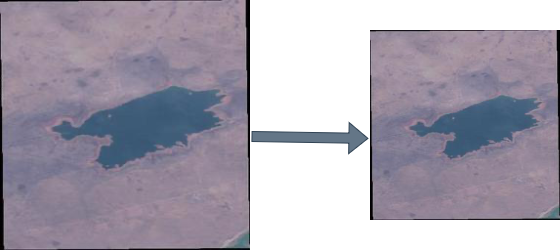
\includegraphics[width= 0.7\textwidth]{figs/resize.png}
\caption{Resizing from Original image}
\label{res}
\end{figure}


% \begin{figure}[H]
% \centering
% \includegraphics[width=1.06\textwidth]{figs/work.png}
% \caption{Resizing from Original size image}
% \label{res}
% \end{figure}

  
  
  \item \textbf{Normalization: }In our thesis, various normalization techniques are applied to both the input images and the corresponding masks. For the images, brightness and contrast adjustments are performed. These adjustments standardize the brightness and contrast levels across the dataset, helping the model to learn more robust features. Additionally, images are rescaled by clipping pixel values to the range of 0 to 255 and casting them to tf.float32, ensuring that the pixel values are in a standard range suitable for processing by the model.\\
  For the mask images, a binary mask creation technique is employed. This involves normalizing the pixel values by setting those greater than or equal to a threshold value (200) to 1 and others to 0. This step is crucial for semantic segmentation tasks as it helps distinguish between the background and the target object, which in this case is the waterbody. By creating binary masks, the model can more effectively learn to segment the water areas.
  
  \item \textbf{Image Augmentation: }Image augmentation is a technique used in data preprocessing to artificially
increase the size and diversity of a dataset by applying various transformations to the original images. It helps improve the generalization and robustness of machine learning models by exposing them to a wider range of
variations and scenarios.Five common types of image augmentation that
have been used in this research are:
 \begin{itemize}
     \item Horizontal Flip: The image is flipped horizontally along the verticalaxis, effectively mirroring it.
     \item The image is flipped vertically along the horizontal axis.
     \item The image is rotated 90 degrees in a clockwise
direction.
\item The image is rotated 180 degrees in a clockwise
direction.

 \end{itemize}
 These augmentation techniques introduce variations in the dataset, enabling
the model to learn features and patterns from different orientations and perspectives. By applying these transformations, the dataset becomes more
diverse, allowing the model to better handle real-world scenarios with variations in orientation, lighting, and other facto
\item \textbf{Conversion to TensorFlow Dataset: }Converting the preprocessed images into a TensorFlow dataset involves transforming the image data into a format that TensorFlow can efficiently use for training machine learning models. 

\end{enumerate} 








\subsection{DCNNs as Backbone with DeepLabV3+}
Utilized ResNet50V2, MobileNetV3, EfficientNetV2 as the backbone architecture for feature extraction, leveraging its pre-trained weights on the ImageNet dataset.\\
Then employed the DeepLabV3+ architecture for semantic segmentation, which incorporates atrous convolution and encoder-decoder structure for capturing contextual information and precise segmentation.\\
The feature maps extracted by these Deep Convolutional Neural Networks (DCNNs) which are used as the backbone network ,serve as
input to the DeepLabV3+ architecture. These feature maps capture rich semantic information from the input images, which is essential for accurate segmentation.
The Below figure \ref{work} shows the graphical representation of the DeepLabv3+ model with DCNN backbone. \\

\begin{figure}[H]
\centering
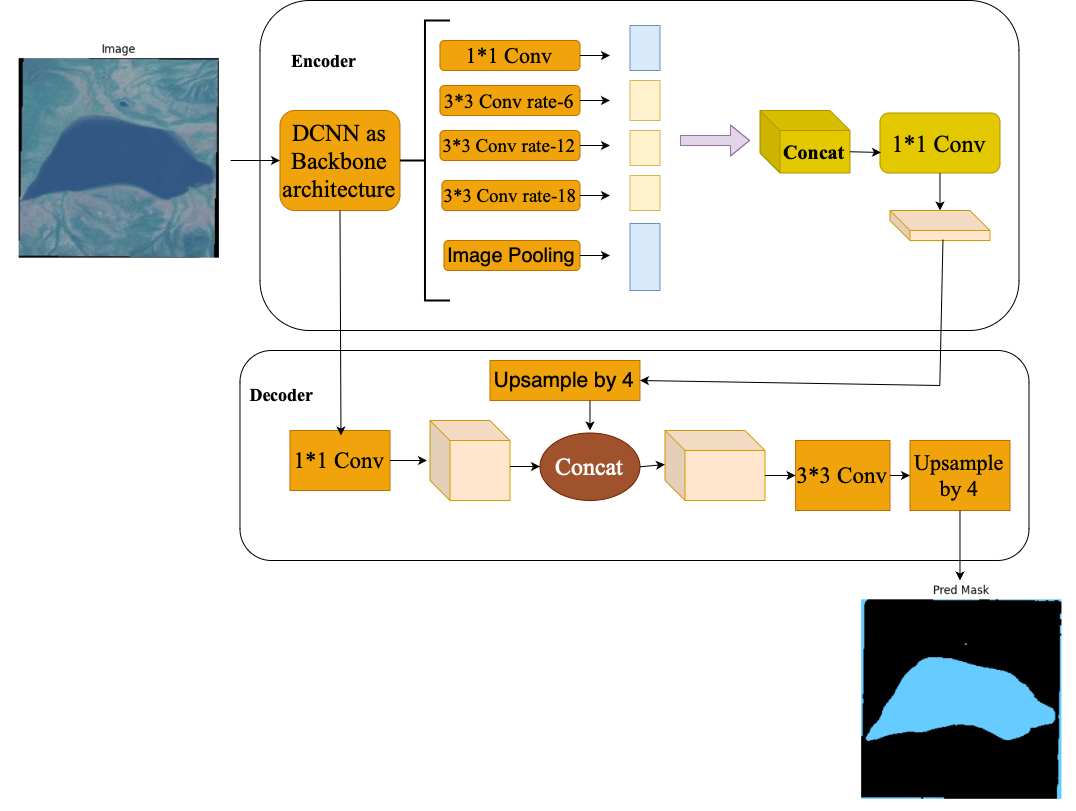
\includegraphics[width=1.06\textwidth]{figs/deeplab.png}
\caption{Proposed DeepLabv3+ Model with DCNN as Backbone}
\label{work}
\end{figure}

\subsubsection{Key Components of the Deeplabv3+ Model}
\begin{enumerate}
    \item \textbf{Atrous (Dilated) Convolutions: }DeepLabV3+ with a DCNN backbone utilizes atrous convolutions to capture multi-scale contextual information without down-sampling the feature maps.Atrous convolutions with different dilation rates are employed to capture features at multiple scales, enabling the model to effectively segment objects of various sizes.

    \item \textbf{Atrous Spatial Pyramid Pooling (ASPP): }The ASPP module aggregates contextual information from multiple scales using atrous convolutions with different rates.It enhances the network's ability to capture both local and global context, which is crucial for accurate semantic segmentation.
    \item \textbf{Decoder Module: }The decoder module refines the segmentation predictions obtained from the ASPP module by restoring spatial details and integrating high-level semantic information.t includes upsampling layers to restore the spatial resolution of the feature maps and fusion layers to combine semantic information from the ASPP module with detailed spatial information.
    \item \textbf{Upsampling: }It is the Bilinear interpolation to upsample the feature maps.Skip connections from earlier layers in the encoder to combine high-resolution features.This module upsamples the low-resolution feature maps obtained from the encoder to the original image resolution.
    \item \textbf{Final Classification Layer: }It applies a 1x1 convolution to produce the final segmentation map with the desired water bodies and non-water bodies classes.The final classification layer produces pixel-wise segmentation predictions. It typically consists of a convolutional layer with softmax activation, assigning a probability distribution to each pixel across different classes e.g., water bodies and non-water bodies.The segmentation masks generated by this layer delineate the extent of water regions in the input imagery.
\end{enumerate}

By integrating these key components, DeepLabV3+ with a ResNet-50 backbone offers a powerful framework for semantic segmentation, enabling accurate identification and delineation of flood water areas in satellite or aerial imagery.


\subsection{ResNet50V2 Backbone Architecture}
ResNet50 is a widely used convolutional neural network (CNN) that consists of 50 layers. It is part of the ResNet (Residual Network) family \cite{resnet}.The key innovation of ResNet is the introduction of residual learning, which helps in training very deep networks by mitigating the vanishing gradient problem.It is a crucial network for us to understand. It is the basis of much academic research in this field \cite{resnet1}.
The ResNet50V2 model serves as a robust feature extractor in our water bodies segmentation task. By leveraging its deep architecture and pre-trained weights,we can effectively extract rich and hierarchical feature representations from input images, which are crucial for achieving accurate segmentation results in the subsequent stages of our model.
\\
Here is the model architecture of the ResNet50V2 Deep Convolutional neural network in \ref{resnt} \\



\begin{figure}[H]
\centering
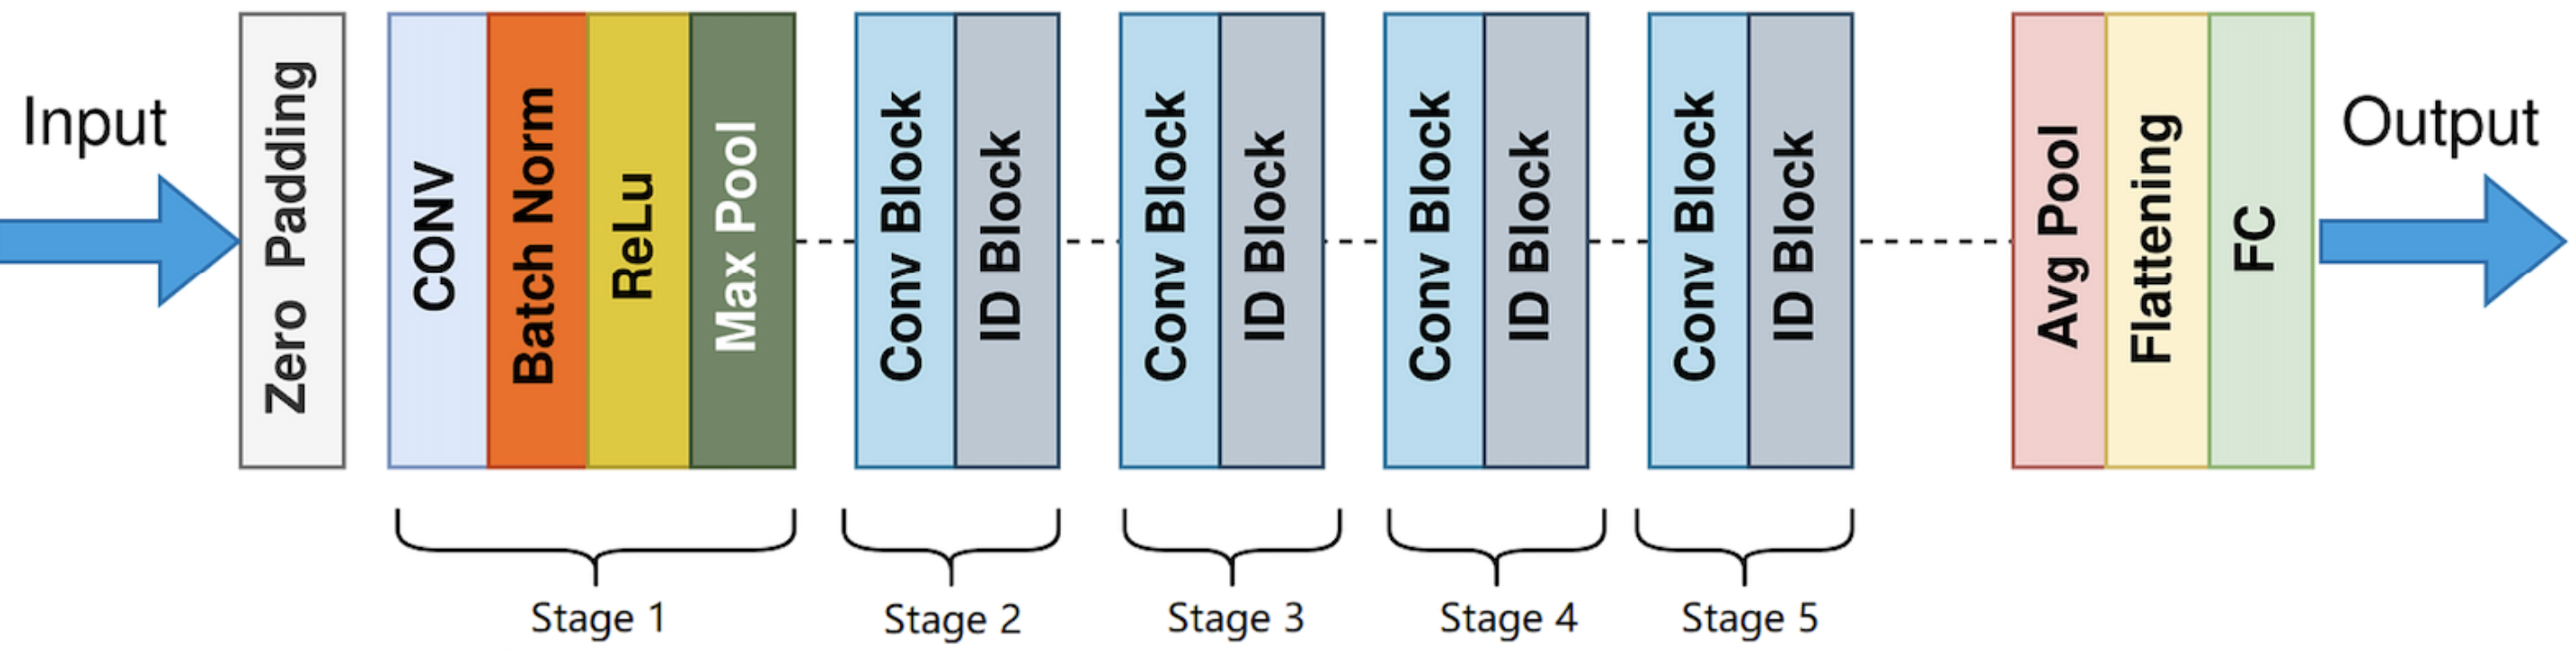
\includegraphics[width=1.05\textwidth]{figs/resnt.png}
\caption{ResNet50 Model Architecture}
\label{resnt}
\end{figure}

\subsubsection{Key Components of ResNet50V2 }
\begin{enumerate}
    \item \textbf{Convolutional Layers: }These layers apply convolution operations to the input images, extracting features through filters that learn spatial hierarchies of features from low to high levels.
    \item \textbf{Residual Blocks: }Residual blocks are the fundamental building units of ResNet. They contain skip connections (or shortcut connections) that bypass one or more layers, allowing the gradient to flow directly through the network, thus facilitating the training of deeper networks.
    \item \textbf{Batch Normalization: }Batch normalization is applied after each convolution layer and before the activation function to stabilize and accelerate the training process by normalizing the inputs to each layer.
    \item \textbf{Activation Functions: }ReLU (Rectified Linear Unit) is used as the activation function, introducing non-linearity into the model and helping it learn complex patterns.
    \item \textbf{Pooling Layers: }Max pooling and average pooling layers are used to downsample the spatial dimensions of the feature maps, reducing the computational complexity and helping in achieving spatial invariance.
    \item \textbf{Fully Connected Layers: }In the context of using ResNet-50 as a feature extractor, the fully connected layers (used for classification in the original network) are typically discarded, and the focus is on using the convolutional layers to extract meaningful feature representations.
    
\end{enumerate}



\subsubsection{Implementation of ResNet50 as a Feature Extractor}
When used as a feature extractor, ResNet50 is responsible for learning and providing rich feature representations from the input images.
\begin{enumerate}
    \item \textbf{Loading the Pre-trained Model:} The pre-trained ResNet-50 model is loaded with weights trained on the ImageNet dataset. This leverages transfer learning, where the model's ability to recognize general features from a large and diverse dataset (ImageNet) is utilized for our specific task of flood water segmentation.
    \item \textbf{Extracting Features: }The feature maps produced by the ResNet-50 backbone are used as input to the DeepLabV3+ architecture. The include-top=False argument ensures that the fully connected layers are not included, focusing on convolutional layers for feature extraction.
    \item \textbf{Integration with DeepLabV3+: }The extracted features are fed into the DeepLabV3+ model, which performs further processing, including atrous spatial pyramid pooling and upsampling, to produce the final segmentation map.
\end{enumerate}


\subsection{MobileNetV3 Backbone Architecture}
MobileNetV3 is a highly efficient neural network architecture designed for mobile applications, making it an excellent choice as a backbone for advanced segmentation models like DeepLabV3+. Its design principles and innovations ensure that it delivers strong performance while being computationally feasible for embedded devices.
By combining MobileNetV3 with DeepLabV3+, we benefit from both the efficiency and powerful feature extraction capabilities of MobileNetV3 and the advanced segmentation techniques of DeepLabV3+, making it well-suited for tasks like water body segmentation.

\subsubsection{Key Components of MobileNetV3}
\begin{enumerate}
    \item \textbf{Depthwise Separable Convolutions: }These convolutions decompose standard convolutions into two simpler operations: depthwise convolutions (which apply a single filter per input channel) and pointwise convolutions.
    This reduces the number of parameters and computational complexity significantly, making the network faster and lighter.

    \item \textbf{Inverted Residuals with Linear Bottlenecks: }This structure preserves information during the transformation, leading to better gradient flow and higher efficiency.

    \item \textbf{Squeeze-and-Excitation (SE) Blocks: }SE blocks help the network to focus on the most informative features, improving the network’s representational power.
    \item \textbf{Neural Architecture Search (NAS): }NAS ensures that the architecture is tailored for both efficiency and high performance, making it suitable for deployment on resource-constrained devices.
\end{enumerate}

\subsubsection{Implementation of MobileNetV3 as Feature Extractor }
Using MobileNetV3 as a feature extractor involves leveraging the pre-trained network's ability to generate rich, hierarchical feature representations from images. This process is essential in transfer learning, where a pre-trained model is adapted to a new task.
\begin{enumerate}
    \item \textbf{Semantic Segmentation: }In semantic segmentation, the feature maps extracted from MobileNetV3 can be used as input to a segmentation head (e.g., ASPP in DeepLabV3+). The segmentation head processes these features to generate a pixel-wise classification map of the input image.
    \item \textbf{Efficiency: }MobileNetV3 is designed to be lightweight and computationally efficient, making it suitable for mobile and embedded devices.
    \item \textbf{Transfer Learning: }Leveraging pre-trained weights from MobileNetV3 allows for effective transfer learning. This means you can benefit from the knowledge the network has already learned from a large dataset like ImageNet.
\end{enumerate}

\subsection{EfficientNetV2 Backbone Architecture}
EfficientNetV2 is a family of convolutional neural networks designed to provide state-of-the-art performance while being computationally efficient. 

\subsubsection{Key Components of EfficientNetV2}
\begin{enumerate}
    \item \textbf{Fused-MBConv Blocks: }The Fused-MBConv block is a new building block in EfficientNetV2, which combines the strengths of MobileNetV2’s MBConv blocks and traditional convolutions.\\
    MBConv is an inverted residual block with a depthwise separable convolution and an expansion phase.
    Fused Convolution Combines expansion and depthwise convolution into a single step to reduce memory access and improve efficiency.\\
    It reduces the number of operations and memory footprint, making the model faster and more efficient.
    \item \textbf{ Compound Scaling: }Achieves a better trade-off between model size, speed, and accuracy compared to scaling only one or two dimensions.
    \item \textbf{Multi-Scale Features: }EfficientNetV2 is designed to capture multi-scale features efficiently, which is crucial for tasks like object detection and semantic segmentation.
\end{enumerate}

\subsubsection{Implementation of EfficientNetV2 as Feature Extractor}
Using EfficientNetV2 as a feature extractor involves leveraging its pre-trained convolutional layers to generate rich feature representations from input images.

\begin{enumerate}
    \item \textbf{Load the Pre-trained EfficientNetV2 Model: }EfficientNetV2 can be loaded with pre-trained weights, usually on ImageNet to take advantage of the learned features. 
    \item \textbf{Extract Features: }The output from the last convolutional layer (or an intermediate layer) of EfficientNetV2 is used as the feature representation of the input image.
    
\end{enumerate}






\subsection{Training Details}
\begin{enumerate}
    \item \textbf{Hyperparameters and Configurations:}
    \begin{itemize}
        \item \textbf{Batch Size: }The number of samples processed before the model is updated. A batch size of 8 was chosen to balance memory usage and convergence speed.
        \item \textbf{Epochs: }The number of complete passes through the training dataset. The model was trained for 45 epochs to ensure sufficient learning.
        \item \textbf{Learning Rate: }The step size at each iteration while moving toward a minimum of the loss function. An initial learning rate of 0.001 was used, with a learning rate scheduler to reduce the rate.
    \end{itemize}
    \item \textbf{Optimizer}
    \begin{itemize}
        \item \textbf{Adam Optimizer: }Combines the advantages of two other extensions of stochastic gradient descent. Adam optimizer was chosen for its efficiency and effectiveness in handling sparse gradients.
    \end{itemize}
    \item \textbf{Callbacks}
    \begin{itemize}
        \item \textbf{Early Stopping: }Monitors the validation loss and stops training when it has not improved for 10 consecutive epochs. This helps prevent overfitting and unnecessary training time.
        \item \textbf{Model Checkpoint: }Saves the best model based on validation accuracy. This ensures the best performing model is retained.
        \item \textbf{Learning Rate Scheduler: }Reduces the learning rate by a factor of 0.1 if the validation loss does not improve for 5 consecutive epochs. This helps in fine-tuning the model during training.
    \end{itemize}
    \item \textbf{Normalization and Regularization}
    \begin{itemize}
        \item \textbf{Batch Normalization: }Applied to improve the training speed and stability of the neural network. It normalizes the input of each layer to have zero mean and unit variance.
        % \item \textbf{Dropout: }A dropout layer with a dropout rate of 0.5 was used to prevent overfitting by randomly setting a fraction of input units to 0 during training.
    
    \end{itemize}
\end{enumerate}

\subsection{Evaluation of the Model}

\begin{itemize}
   
        \item The training was monitored using the validation dataset to adjust parameters and prevent overfitting.
        
    \end{itemize}
    These configurations and techniques collectively ensure the model's effective training and generalization for the task of water bodies segmentation. The figure \ref{predict2} below shows the images after training and evaluation of the remote sensing images.


\begin{figure}[H]
\centering
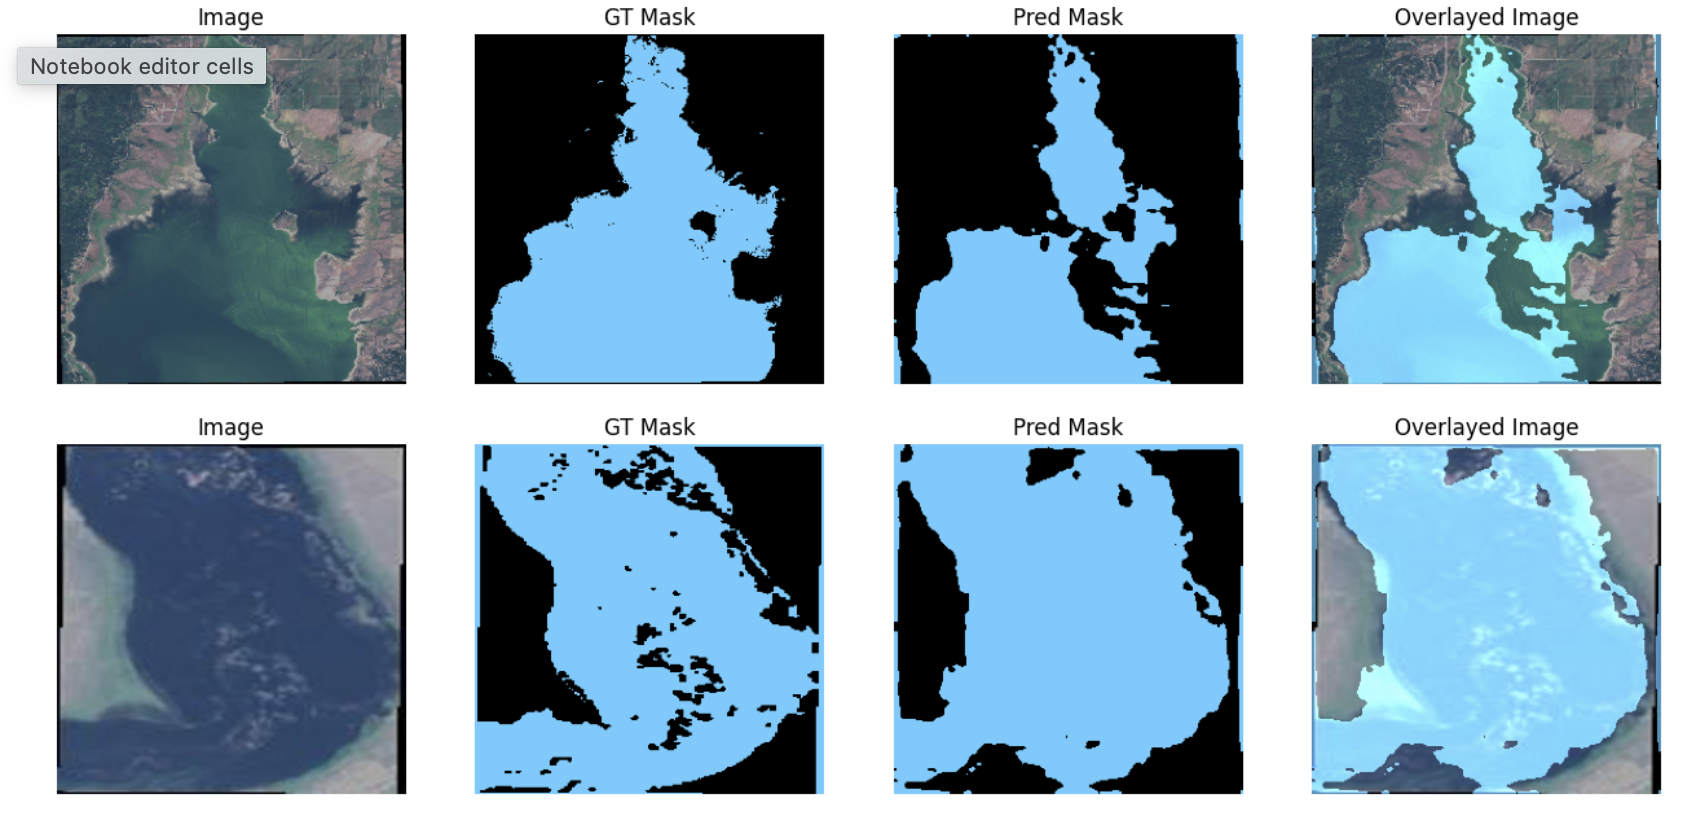
\includegraphics[width=0.9\textwidth]{figs/predict.png}
% \caption{Result of the input images after evaluation(1)}
\label{predict1}
\end{figure}

\begin{figure}[H]
\centering
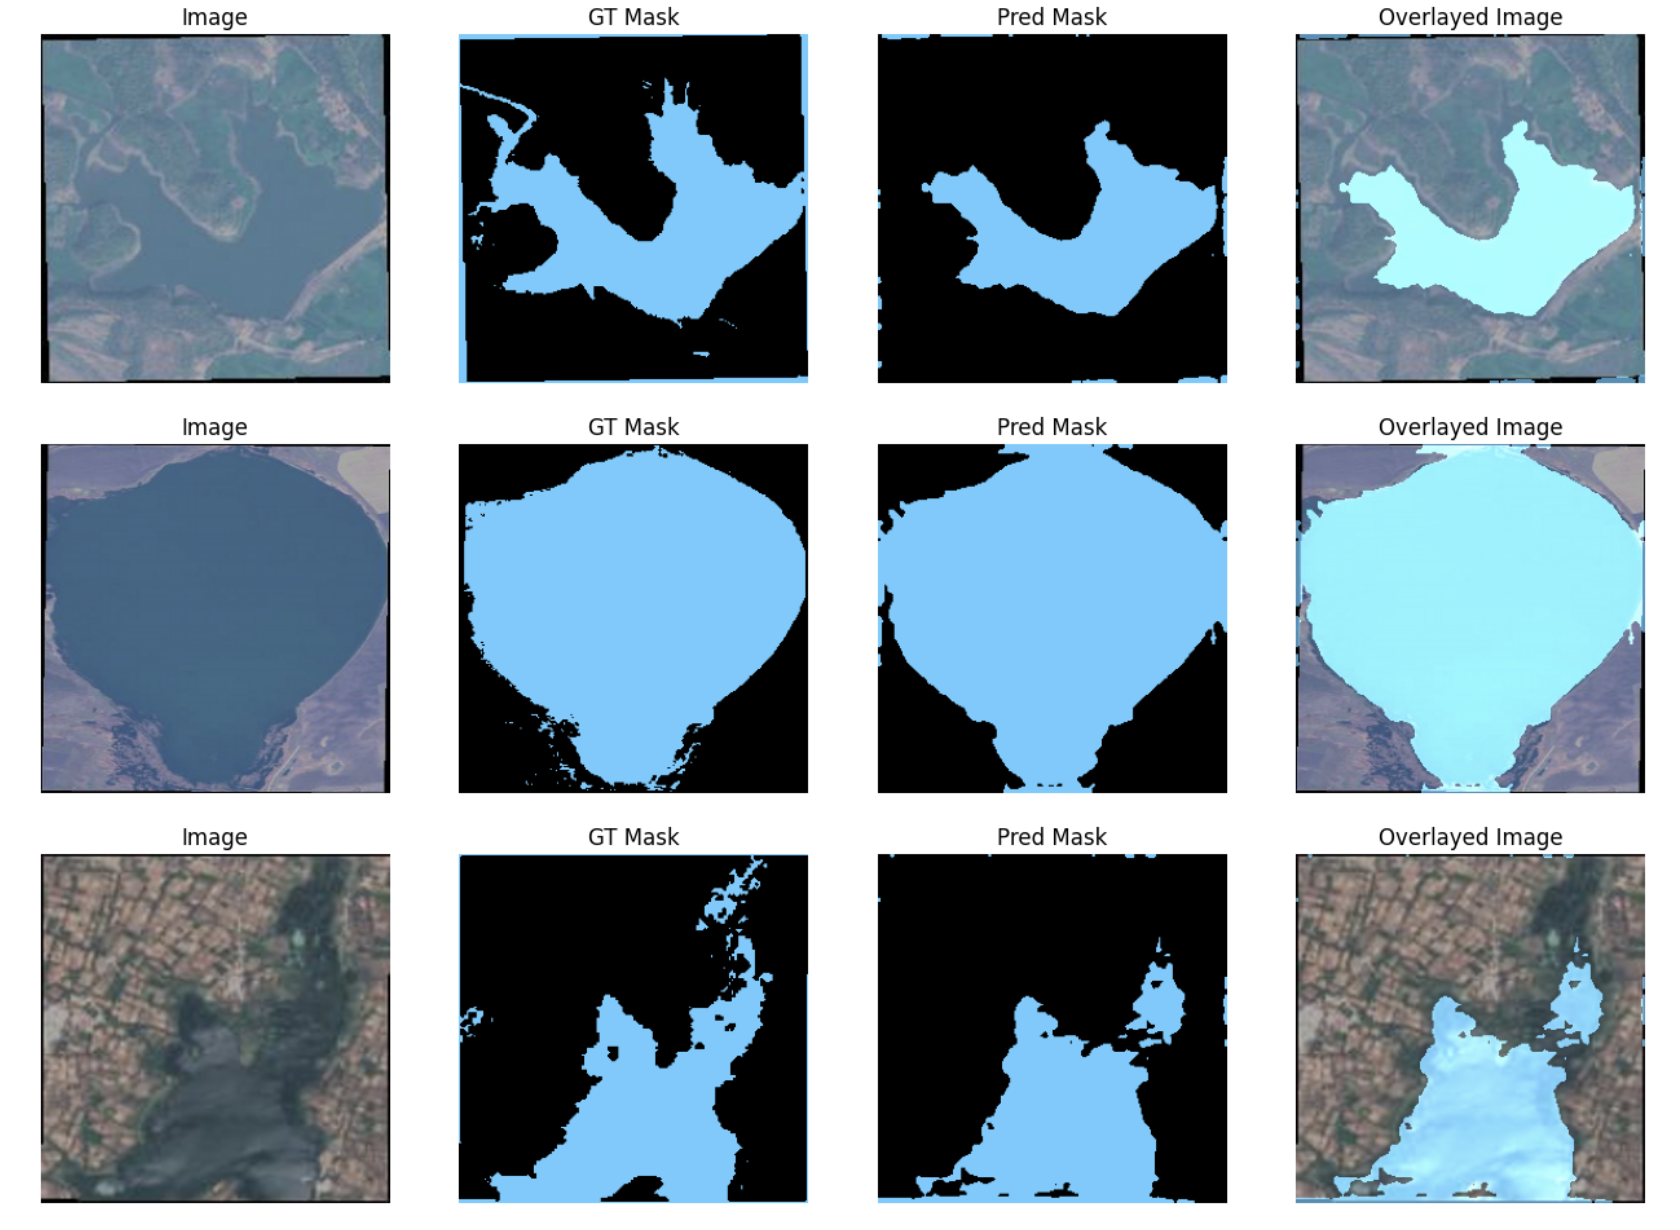
\includegraphics[width=1\textwidth]{figs/evaluation.png}
\caption{Result of the input images after evaluation}
\label{predict2}
\end{figure}



\section{Conclusion}
In this chapter, a detailed explanation of the proposed methodology is provided and then demonstrated its implementation. The full methodology was divided into four parts: Data preprocessing,Deeplabv3+ model with DCNNs as backbone, Training Details and Evaluation the model. The following chapter is organised with the results and outcomes of our proposed model with necessary explanation and analysis. The results and effectiveness of our method will be described in the following chapter.